\documentclass[aspectratio=169, 14pt]{beamer}

\makeatletter
\def\input@path{{usyd-beamer-theme/}}
\makeatother

\usepackage{amsmath}
\usepackage{fontspec}

\defaultfontfeatures{Extension = .otf}% adds .otf to end of path when font loaded without ext parameter e.g. \newfontfamily{\FA}{FontAwesome} > \newfontfamily{\FA}{FontAwesome.otf}
\usepackage{fontawesome}

\usepackage{color}
\usepackage{listings}
\usepackage[lighttt]{lmodern}

% Defining colours based on HUSL scheme
% all colours have same saturation (100) and luminance (30)
\definecolor{myred}{rgb}{0.37938,0.25242,0.00000}
\definecolor{myyellow}{rgb}{0.34018,0.26948,0.00000}
\definecolor{mygreen}{rgb}{0.00000,0.32236,0.16680}
\definecolor{myblue}{rgb}{0.00000,0.28379,0.50129}
\definecolor{mypurple}{rgb}{0.47903,0.00000,0.57397}
\definecolor{mygrey}{rgb}{0.27699,0.27699,0.27699}

\lstset{%
    backgroundcolor=\color{white},  % Background colour
    basicstyle=\ttfamily,            % Standard font settings
    breaklines=false,                % Automatic line breaking, only at whitespace
    captionpos=b,                   % Sets caption position to bottom
    commentstyle=\color{mygrey},    % Set comment colour
    keywordstyle=[1]\color{mypurple},  % Keyword style
    keywordstyle=[2]\color{mygreen},  % Keyword style
    keywordstyle=[3]\color{myblue},  % Keyword style
    stringstyle=\color{myred}      % String colour
}

\title{\large Learning from Machine Learning}
\date{\today}
\author[Malcolm]{Malcolm Ramsay \\ \faTwitter~@malramsay64 \\ \faGithub~malramsay64}

\usetheme{usyd}
% To use the logobar theme use the line below instead
% \usetheme[logobar]{usyd}

\titlegraphic{config_crop.png}
\titlegraphicbackground{usydred}

\graphicspath{{usyd-beamer-theme/}{figures/}}

\begin{document}

\begin{frame}
  {\fontsize{12}{14}\selectfont
  \titlepage{}
}
\end{frame}

\section{Machine Learning}
\begin{frame}{What is Machine Learning?}

  \begin{itemize}
    \item Technique for drawing a line
    \item Complicated methods draw complicated lines
  \end{itemize}

  \begin{columns}
    \begin{column}{0.5\textwidth}
      \includegraphics<2->[width=\textwidth]{drawing_lines_regression}
    \end{column}
    \begin{column}{0.5\textwidth}
      \includegraphics<3->[width=\textwidth]{drawing_lines_classification}
    \end{column}
  \end{columns}

\end{frame}

\begin{frame}[label=follow-along]{Follow along}

  \begin{center}
    \LARGE
    \url{demo.malramsay.com}
  \end{center}

  \begin{itemize}
    \item Shift + Enter to run code
    \item Run all cells from the top
  \end{itemize}

  All code and more available at \\
  \url{github.com/malramsay64/MLCrystals}

\end{frame}


\begin{frame}{}

  \color{usydred}
  \LARGE
  What makes Machine Learning easy?

\end{frame}


\begin{frame}{Standard Datasets}

  \begin{columns}
    \begin{column}{0.5\textwidth}
      \begin{itemize}
        \item MNIST Handwritten Digits
        \item ImageNet
        \item Ling-Spam Dataset of emails
      \end{itemize}
    \end{column}
    \begin{column}{0.5\textwidth}
      \center
      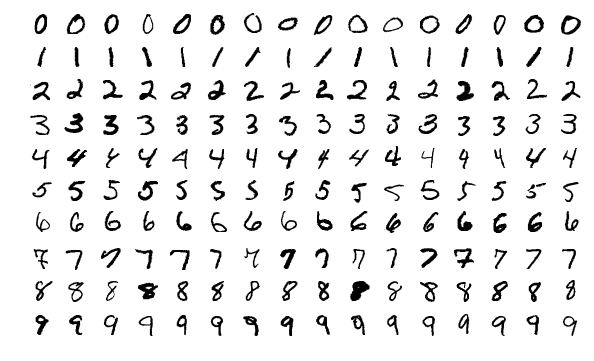
\includegraphics[height=5em]{mnist_examples}
      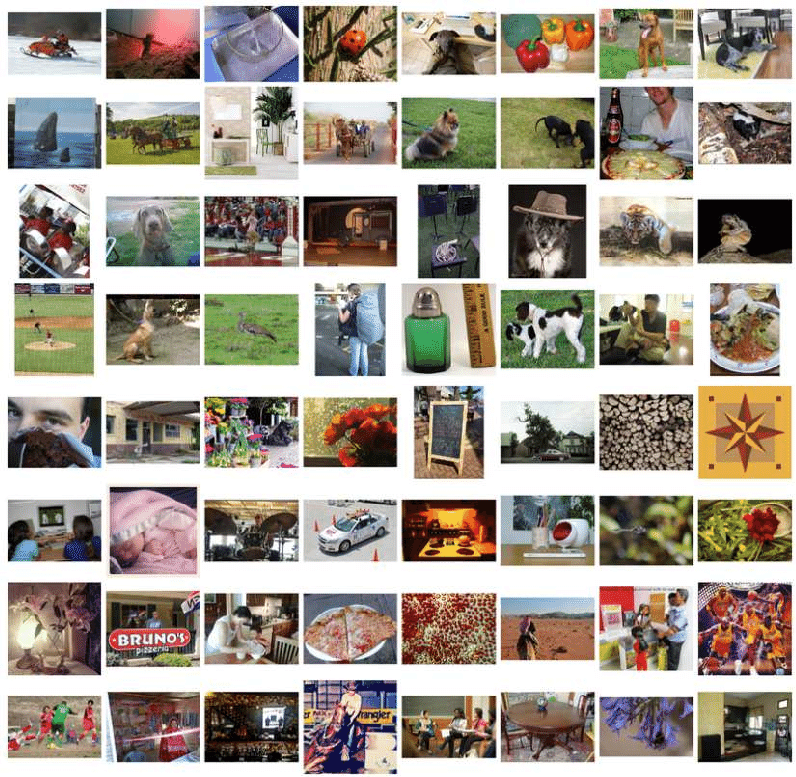
\includegraphics[height=7em]{imagenet_examples}
    \end{column}
  \end{columns}

\end{frame}


\begin{frame}{Sharing of all code}

  \begin{itemize}
    \item Highly competitive field
    \item Even from commercial entities
    \item Code is a way of getting your paper noticed
  \end{itemize}

\end{frame}


\begin{frame}[fragile]{Is using Open Source Libraries enough}

  \begin{columns}
    \begin{column}{0.7\textwidth}
      \scriptsize
      \begin{lstlisting}[language=python]
import hoomd
from hoomd import md
hoomd.context.initialize()

# create a 10x-axis square lattice of particles with name A
hoomd.init.create_lattice(unitcell=hoomd.lattice.sc(a=2.0, type_name='A'), n=10)
# specify Lennard-Jones interactions between particle pairs
nl = md.nlist.cell()
lj = md.pair.lj(r_cut=3.0, nlist=nl)
lj.pair_coeff.set('A', 'A', epsilon=1.0, sigma=1.0)
# integrate at constant temperature
all = hoomd.group.all();
md.integrate.mode_standard(dt=0.005)
hoomd.md.integrate.langevin(group=all, kT=1.2, seed=4)
# run 10,000 time steps
hoomd.run(10e3)
      \end{lstlisting}
    \end{column}

    \begin{column}{0.3\textwidth}
      \vspace{3em}
      \begin{itemize}
        \item 12 parameters
        \item 11 lines of code
      \end{itemize}
    \end{column}
  \end{columns}

\end{frame}


\begin{frame}{Easy to get started}
  \begin{itemize}
    \item Interactive tutorials (\url{kaggle.com/learn})
    \item Browser based tools (\url{colab.research.google.com})
    \item Simple installation processes
  \end{itemize}
\end{frame}


\begin{frame}{}

  \color{usydred}
  \LARGE
  What does this look like in Statistical Dynamics?

\end{frame}

\againframe{follow-along}

\begin{frame}{Trimer Model}

  \begin{columns}
    \begin{column}{0.4\textwidth}
      \begin{itemize}
        \item 2D rigid molecules
        \item Molecular Dynamics simulations
      \end{itemize}
    \end{column}
    \begin{column}{0.6\textwidth}
      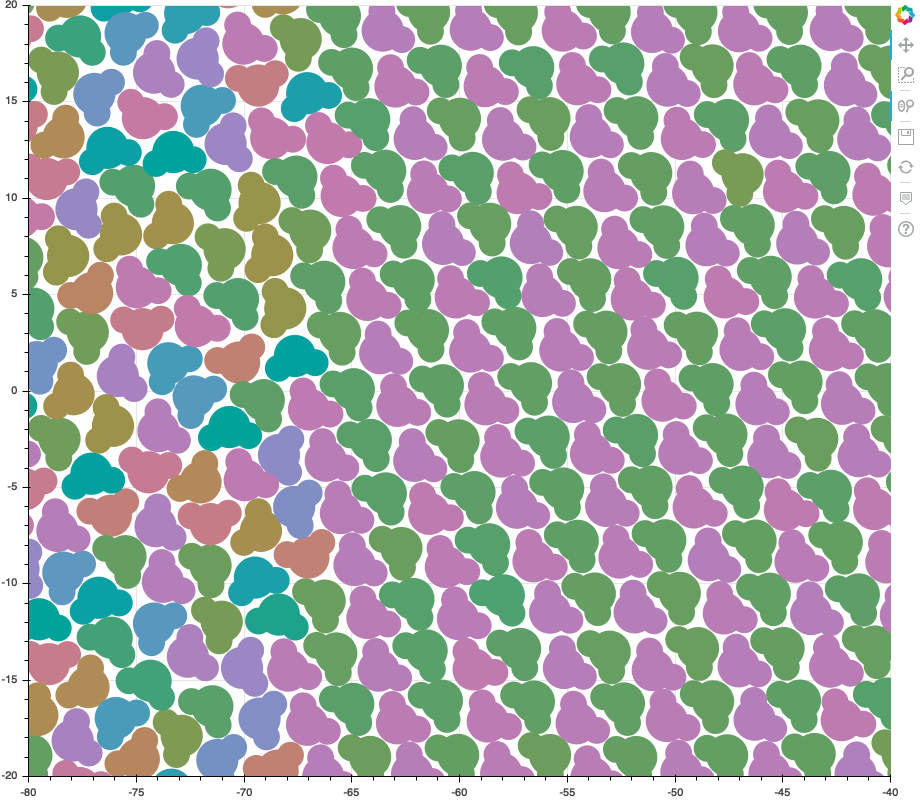
\includegraphics[width=\textwidth]{Trimer_snapshot.png}
    \end{column}
  \end{columns}
\end{frame}


\begin{frame}{Features in Trimer Model}

  \begin{columns}
    \begin{column}{0.5\textwidth}
      \begin{itemize}
        \item Relative orientation of nearest neighbours
        \item Invariant of crystal orientation
      \end{itemize}
    \end{column}
    \begin{column}{0.5\textwidth}
      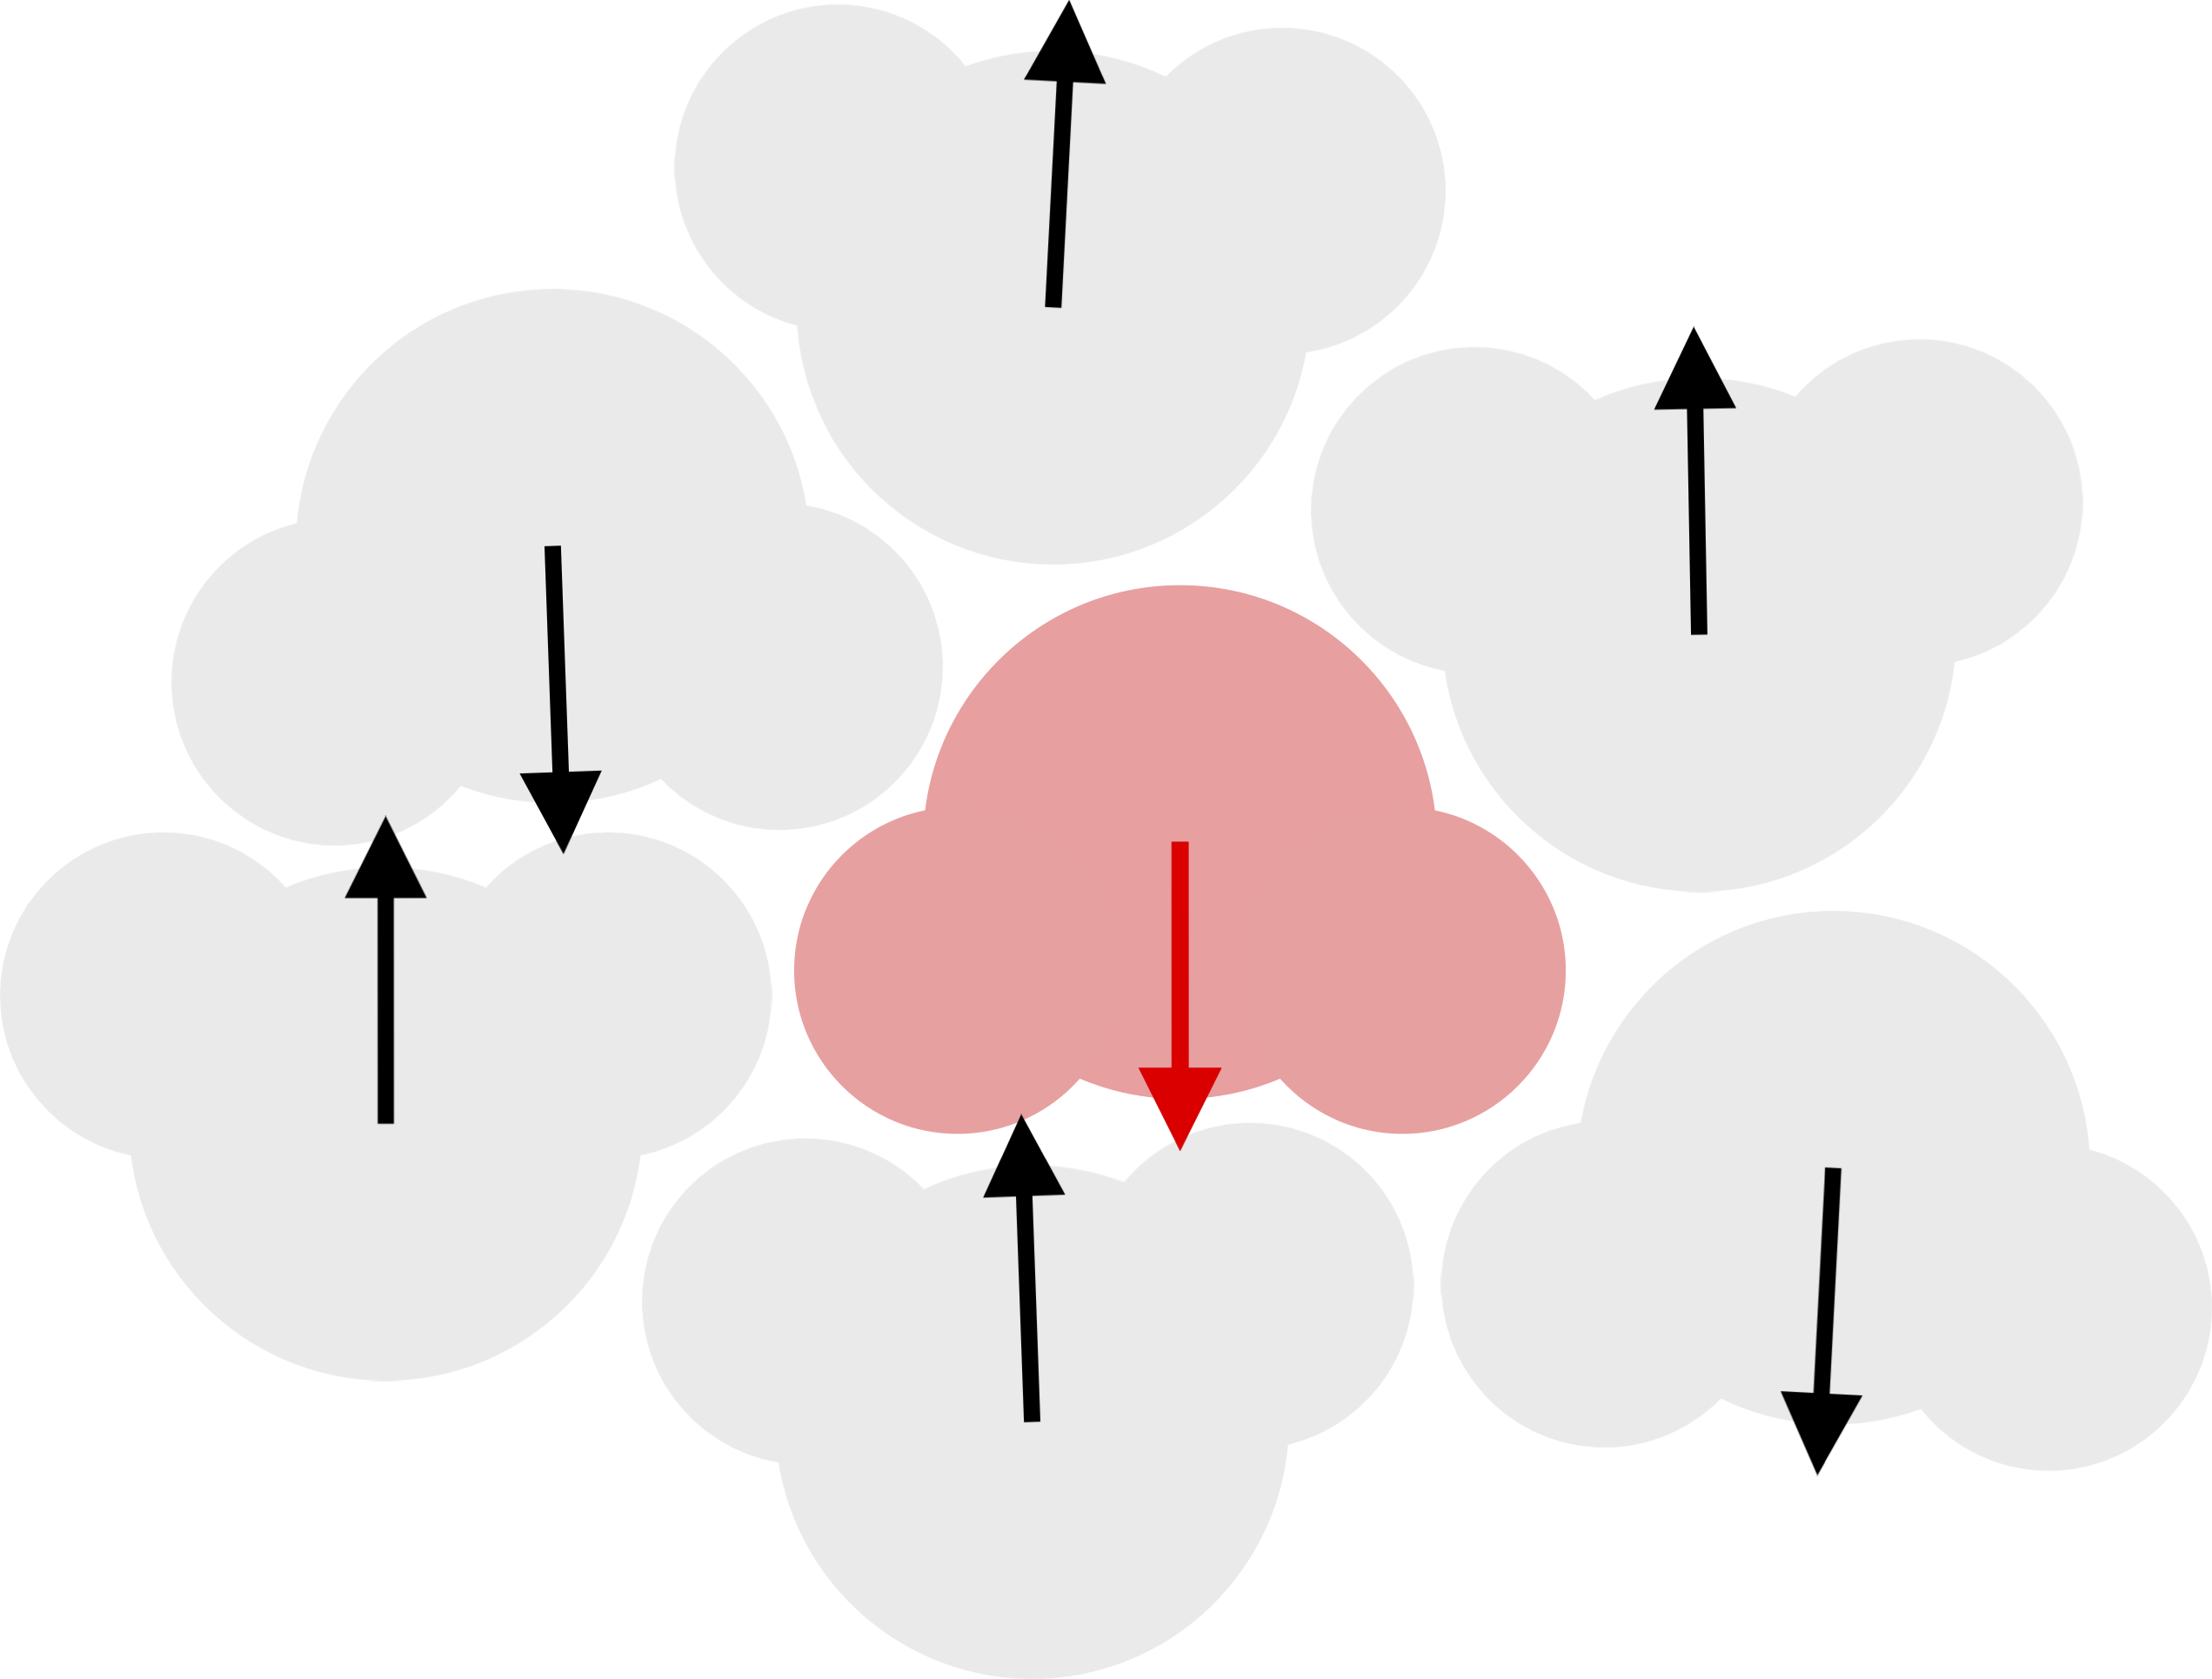
\includegraphics[width=\textwidth]{orientations.png}
    \end{column}
  \end{columns}
\end{frame}


\section{Machine Learning}
\begin{frame}{Machine Learning}

  \begin{itemize}
    \item Create a dataset of correctly labelled values
    \item Split data set
      \begin{itemize}
        \item 80\% Training
        \item 20\% Test
      \end{itemize}
    \item Score with the unseen Test dataset
  \end{itemize}

\end{frame}


\begin{frame}{Classification Results}
  \begin{columns}
    \begin{column}{0.33\textwidth}
      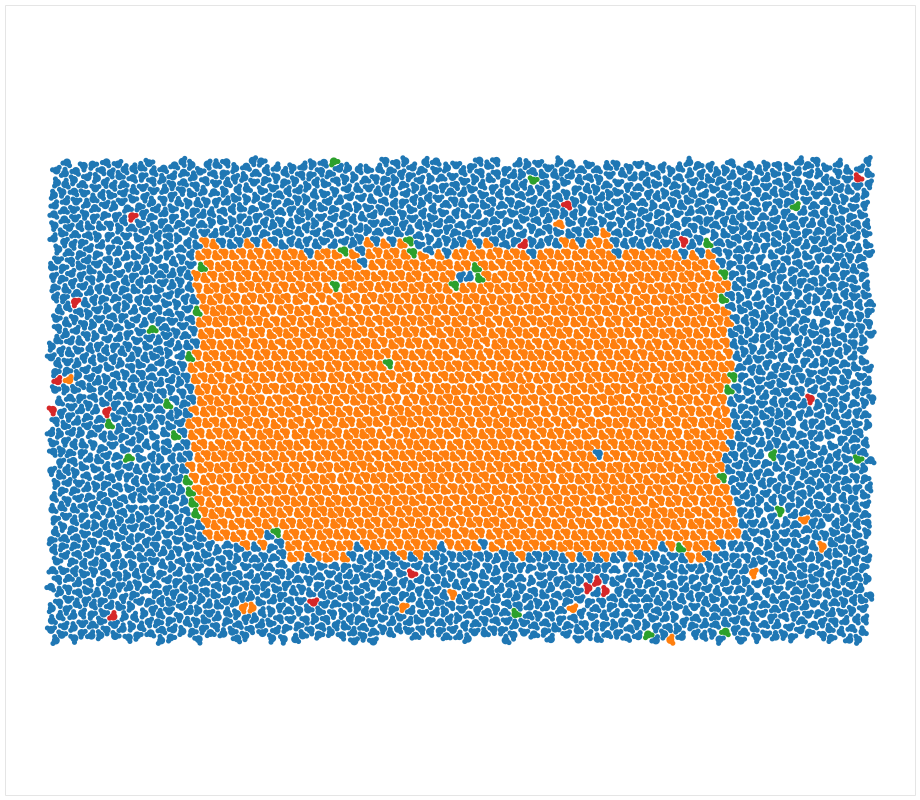
\includegraphics[width=\textwidth]{classification_results_p2.png}
    \end{column}
    \begin{column}{0.33\textwidth}
      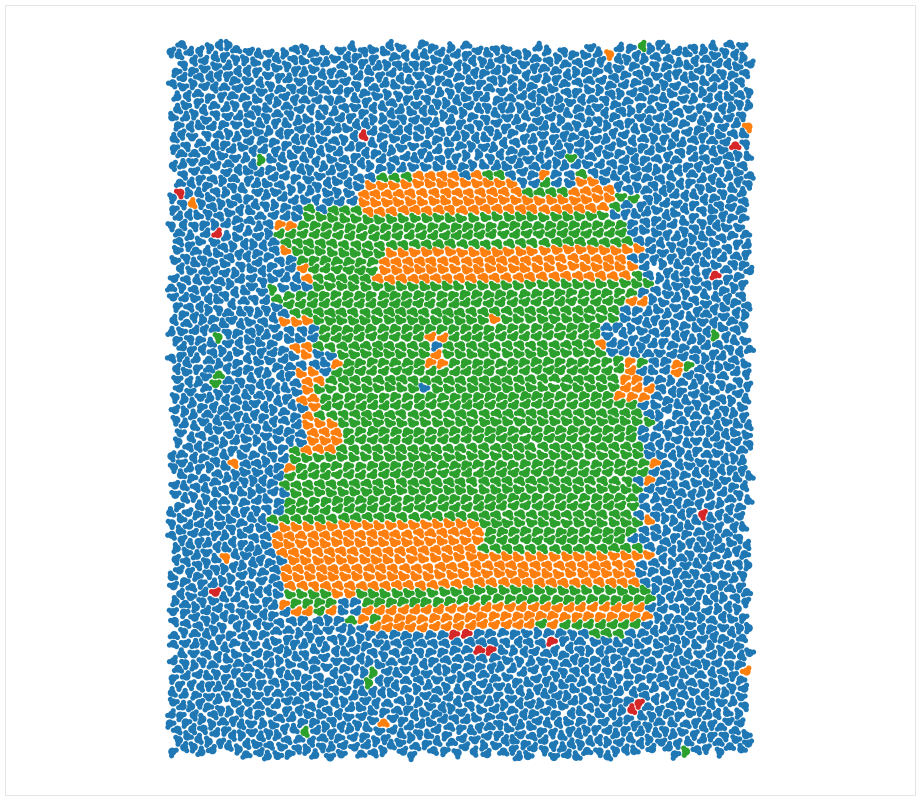
\includegraphics[width=\textwidth]{classification_results_p2gg.png}
    \end{column}
    \begin{column}{0.33\textwidth}
      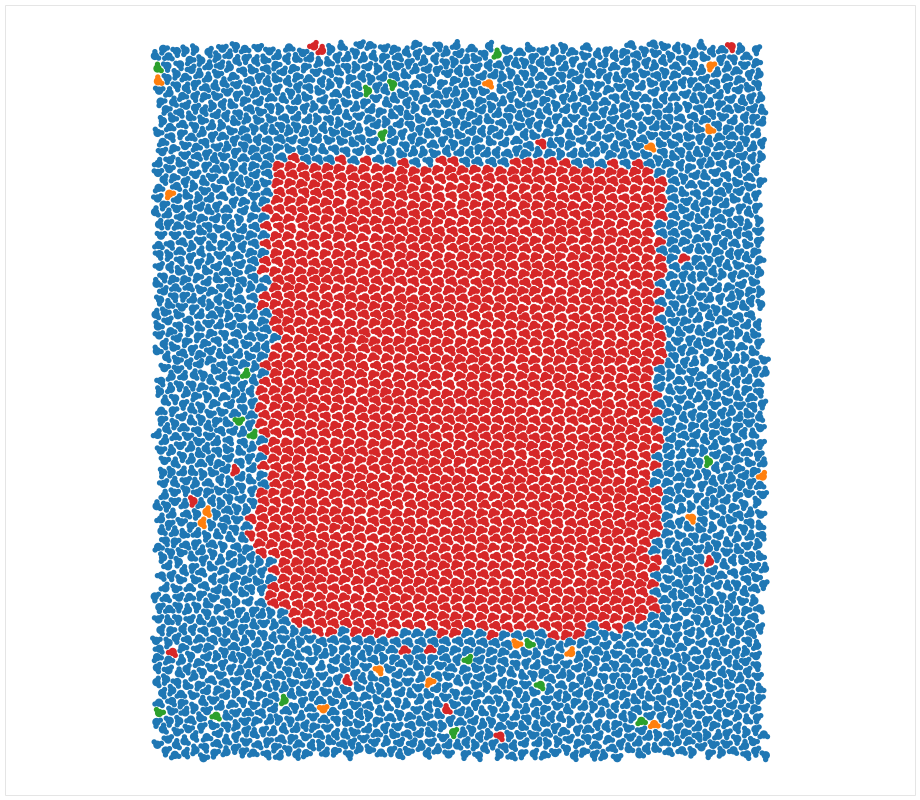
\includegraphics[width=\textwidth]{classification_results_pg.png}
    \end{column}
  \end{columns}
\end{frame}


\begin{frame}{How can we improve?}

  \begin{itemize}
    \item Make datasets freely available
      \begin{itemize}
        \item \item{zenodo.org}
      \end{itemize}
    \item Code is important for anyone replicating your work
      \begin{itemize}
        \item \url{github.com/malramsay64}
      \end{itemize}
    \item Make it easy to get started
      \begin{itemize}
        \item Jupyter Notebooks
        \item \url{mybinder.org}
      \end{itemize}
  \end{itemize}

\end{frame}

\end{document}
